\section{Experiment with Pozyx}
In order to determine the accuracy of the Pozyx tags we conducted an experiment.
The primary goal of the experiment was to test the accuracy, but a by-product of the experiment was to determine the frequencies of updates for each tag.

\subsection{Setup}
The current settings aims to achieve best precision, but gives a smaller amount of updates.
% Uddyb hvilke settings det er og angiv kilde.
The experiment was setup as shown on \autoref{fig:experiment-setup}. 
The experiment was conducted indoors in Novi 9. 
The anchors \texttt{0x632b} and \texttt{0x676e} were mounted on a wall 240 centimeters apart, and the remaining anchors \texttt{0x6738} and \texttt{0x676c} were mounted on a bulletin board.
The number of centimeters accompanying the hexadecimal number of each anchor is the height at which the anchor was mounted during the experiment.
Different heights were chosen as Pozyx documentation suggests that not all anchors should have the same height \cite{pozyx-AnchorHeights}.
The reason for this is the principle of geometric dilution of precision(GDOP), which can cause the error on range measurements to be amplified.

\begin{figure}[H]
    \centering
    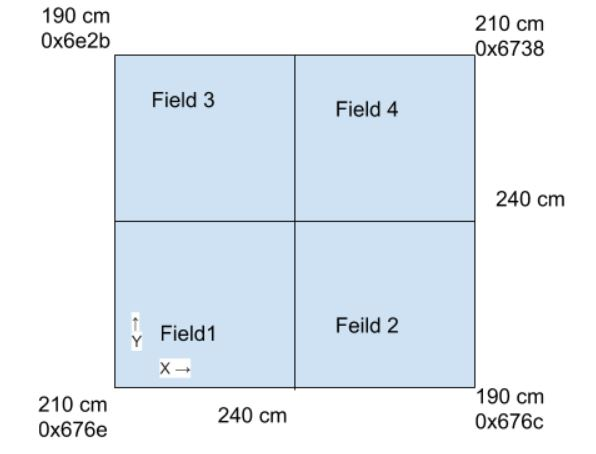
\includegraphics[width=0.6\linewidth]{experiment-setup.JPG}
    \caption{The setup of the experiment with the anchors and the height at which they were placed in the corners.}
    \label{fig:experiment-setup}
\end{figure}
\noindent
The fields were created by a blackboard on which lines were drawn every 10 centimeters to know the actual position as seen on \autoref{fig:experiment-blackboard}.
This blackboard was moved intermittently to act as respectively field 1, field 2, field 3 and field 4.

\begin{figure}[H]
    \centering
    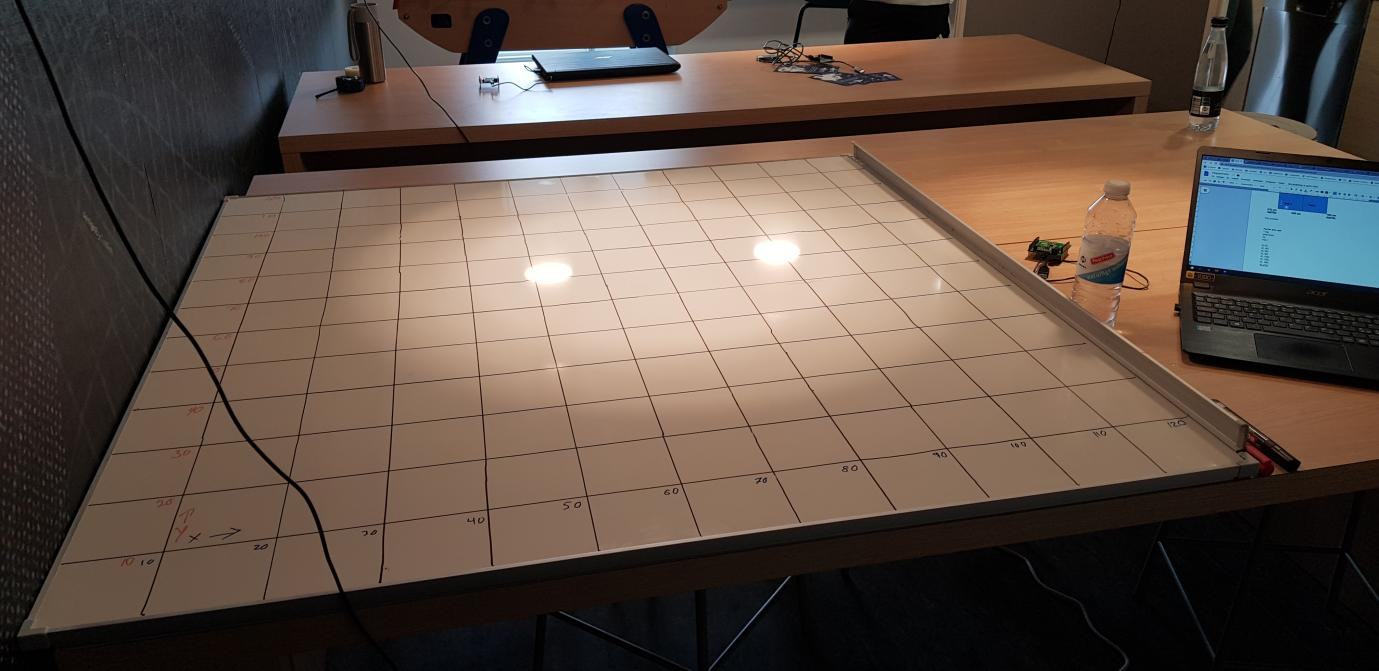
\includegraphics[width=0.8\linewidth]{experiment-blackboard.png}
    \caption{The blackboard with the drawn positions.}
    \label{fig:experiment-blackboard}
\end{figure}
\noindent
The procedure for the experiment was based on this blackboard.
The blackboard would be placed in one of the fields defined in \autoref{fig:experiment-setup}, and we would then place the tags in certain positions on the board and record the accuracy with with the position was reported.
The tags would be placed in a position, remain there for five seconds, then be moved to the next position over the next five seconds and remain in this position for five seconds before being moved again.
This procedure was repeated until a satisfactory number of measurements had been made.
Once one field had been tested, we moved the blackboard to the next field and repeated the setup.
 
\section{Work on the data}
In \autoref{app:experiment} the data for the experiment can be seen.
For each test we calculated the average grid, found the min and max values for \texttt{x}, \texttt{y} and \texttt{z}.
We also calculated the average deviation from the actual grid to the average grid to get a better view of the deviation there was.
The min and max values was noted, as we might need to take this into account. 


\subsection{Precision with 1 tag} 
In \autoref{app:one-tag} can be seen the average grid coordinates, with min and max values.

In \autoref{Tab:average-deviation-1-tag} the average deviation can be seen.
The average of average deviation is 10.54 cm.

\subsection{Precision with 3 tag}
For this part of the experiment we tested the accuracy with 3 tags. 

\subsubsection{Tag 26467}
The overall average deviation for this tag was 11.2 cm.
There were however a large deviation at \texttt{140, 90} and \texttt{(140, 120)} with 20.63 and 20.46 cm.

\subsubsection{Tag 26895}
The overall average deviation for this tag was 6.31 cm.
The average deviation was more accurate than expected for this tag.

\subsubsection{Tag 24622}
The overall average deviation for this tag was 17.41.
The first three points we tried out seemed fairly accurate, however the grid \texttt{(220, 90)} and \texttt{(220, 120)} had a large deviation of 37.53 cm and 24.4 cm.

\subsection{Precision with 5 tag}
For this experiment we have also noted how many data points there were sent in the 5 second intervals, as well as the average deviation

\subsubsection{Tag 24622}
The average deviation for this tag was 8.42 cm and the average amount of data points each 5 seconds was around 4.28 data points.
However, at \texttt{(180, 120)} we only recieved 1 data point.

\subsubsection{Tag 26895}


\subsubsection{Tag 26467}


\subsubsection{Tag 26901}


\subsubsection{Tag 27001}

\subsection{Possible influences on the test}
One thing that could have affected the tags is that we used a blackboard as a measure for positions. 
As there is metal in the blackboard this could have affected the precision on the tags.
Metals are conductors, which can lead to the signal having less power and reduced range, and the signal might spend extra time trying to get through the metal.
Since Pozyx positioning relies on calculating the time of flight, having the signal spend extra time travelling reduces accuracy \cite{pozyx-UWBObstacles}. 
\\\\
During the test with 1 tag, the 0 value of the $x$ coordinate coincided with the wall. 
This could have been an influence on the positing result in that it could increase uncertainty, as it was difficult to center the tag over the x coordinate since the coordinate collided with the wall.

\subsection{Conclusion on the experiment}